\mychapter{Réécriture}
\label{Cap:TD1}


\section{Description physique}
Nous avons decrit physiquement le système demandé sur la gestion d’une voie de péage d’autoroute.
\begin{figure}[h]
    \centering
    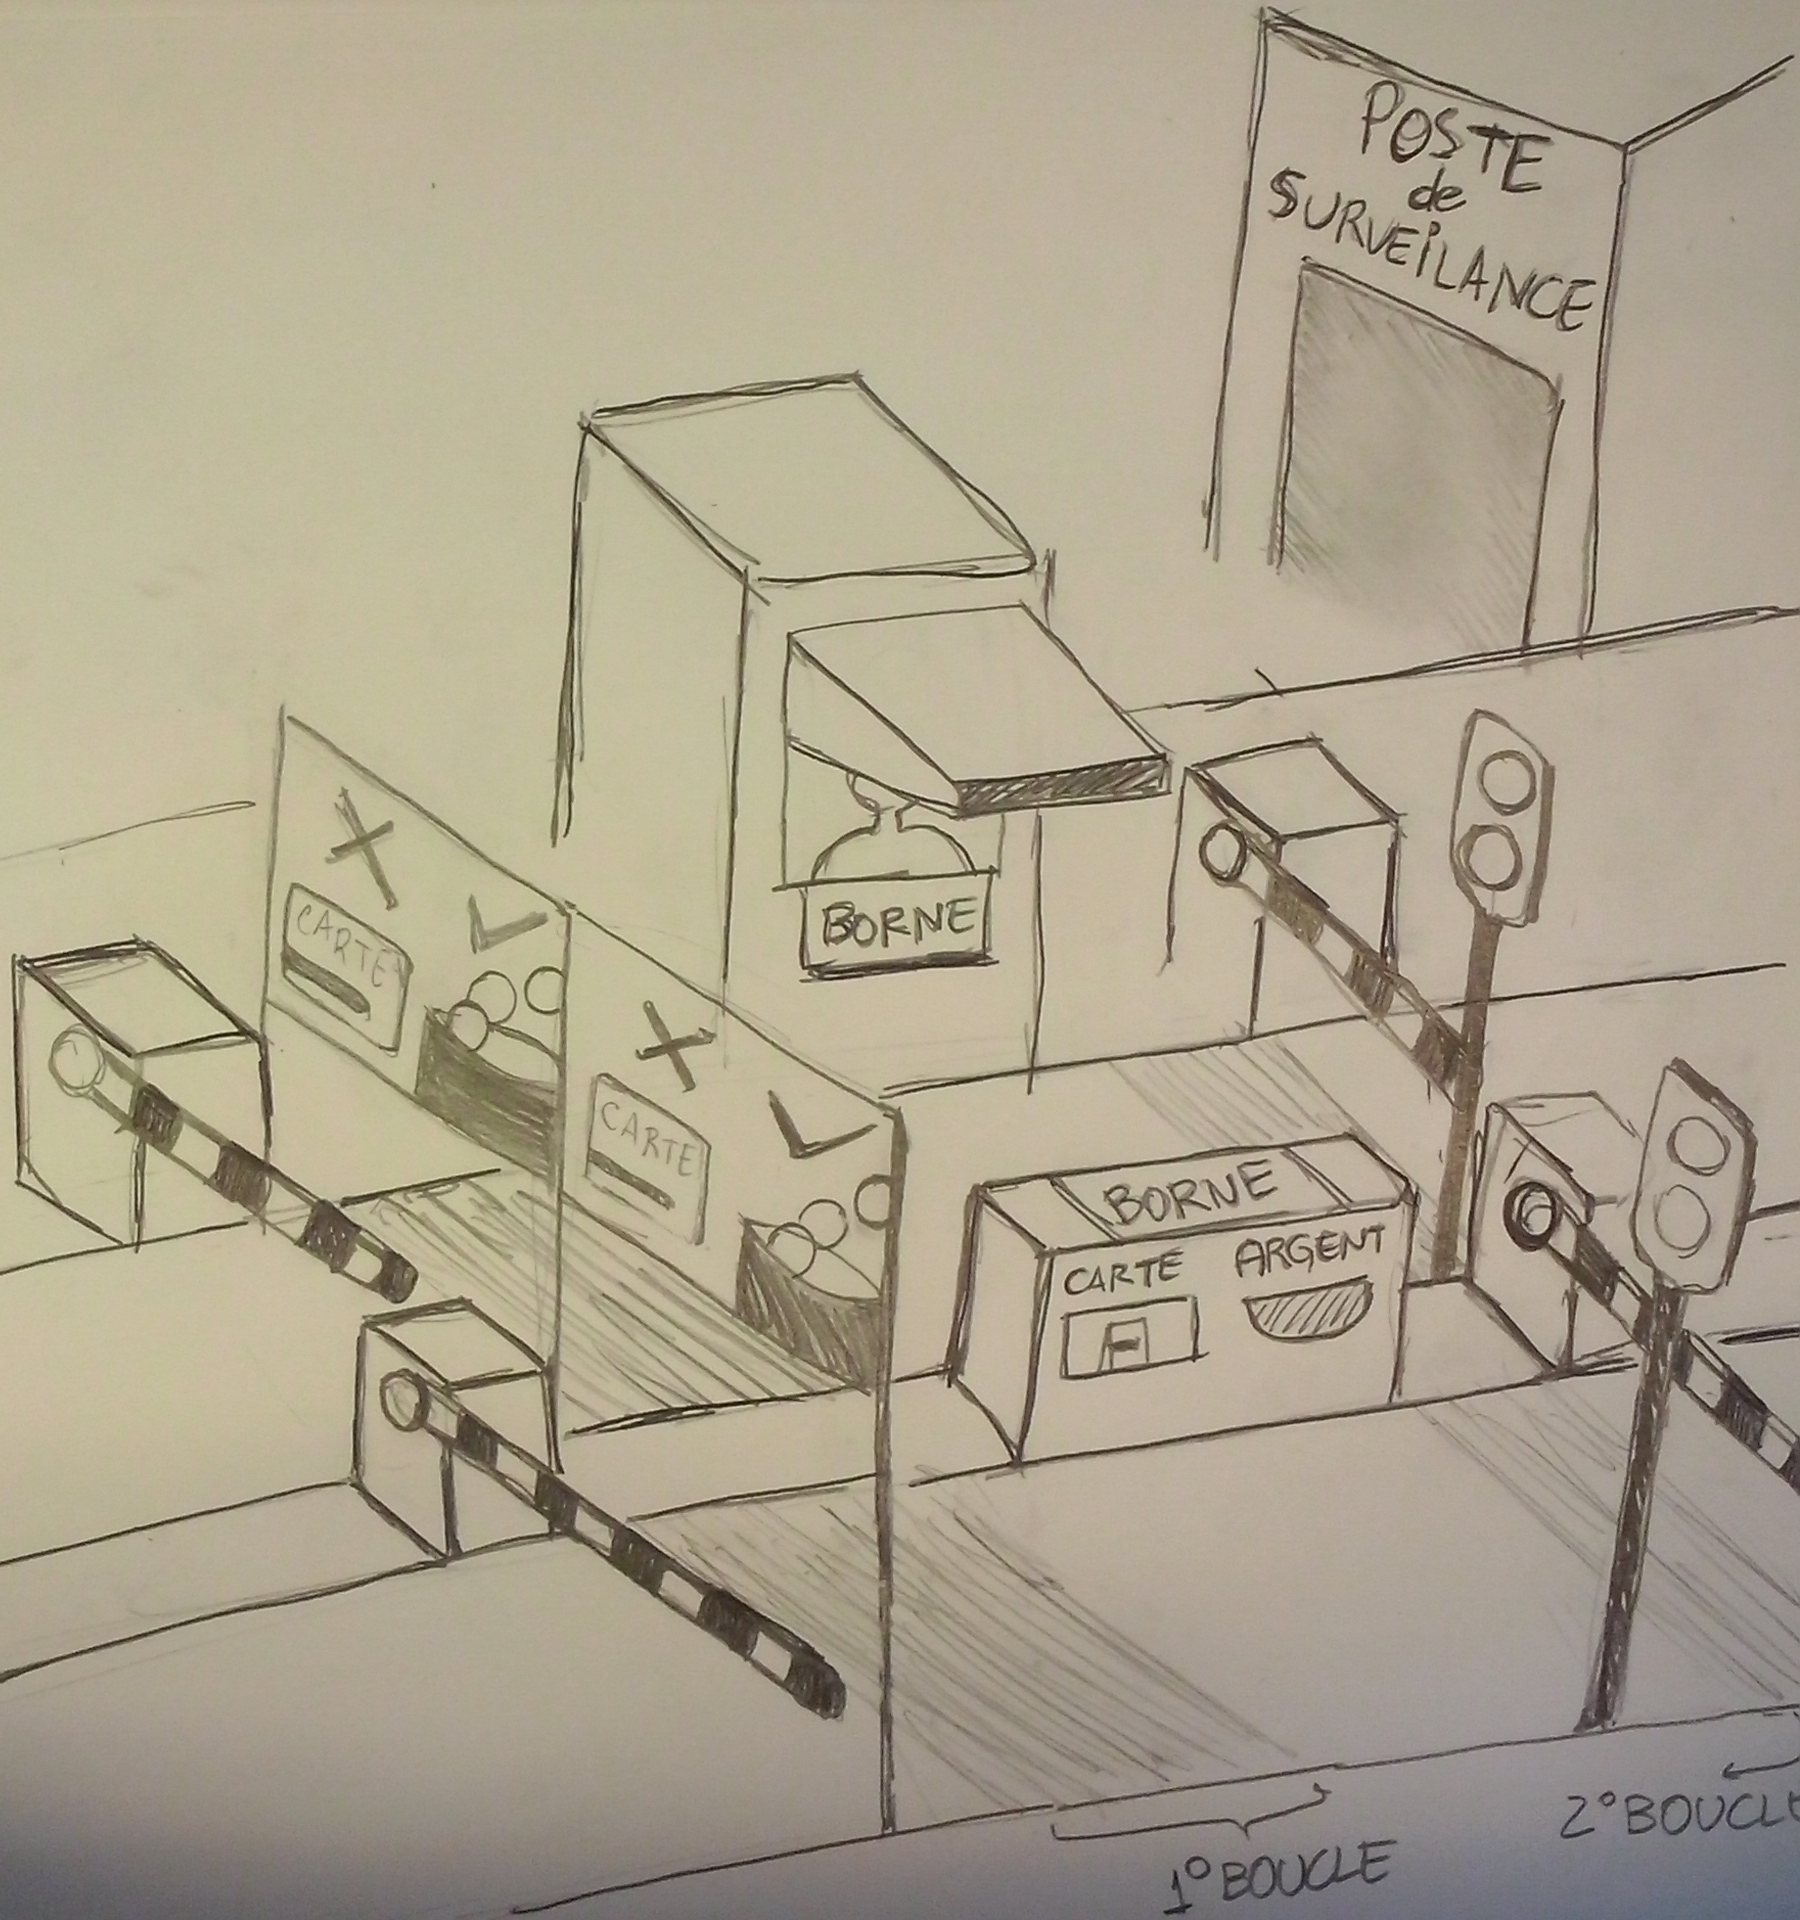
\includegraphics[scale=0.2]{02_Desenvolvimento/TD1/images/image.png}
    \caption{Description physique}
\end{figure}
\newpage
\textbf{Légende}
\begin{enumerate}
    \item Exemple d'une borne automatique
    \item Exemple d'une borne manuelle, où l'usager paye à un opérateur humain.
    \item Poste de surveillance, où les surveillants sont.
\end{enumerate}
    \textbf{Observation sur les borne}: Il y a autres différents types de borne, au total sont: 
    \begin{itemize}
        \item Borne Manuelle, où l'usager paye via un opérateur humain.
        \item Borne automatique où l'usager paye soit en pièces dans un appareil capable de rendre la monnaie si nécessaire, soit avec une carte d'abonnement soit avec une carte de crédit.
        \item Borne de télepeage qui détecte automatiquement la présence d'une carte affiché sur le véhicule et déclenche le changement de couleur du feu et le lever de barrieère.
        \item Borne mixte autorisant le paiement automatique et le télépeage.
    \end{itemize}
\newpage
\section{Réécriture de l'expression des besoins recentrée sur les utilisateurs du systeme}
\subsection{Les acteurs} 
Nous avons reconnu cinq acteurs (utilisateurs) du système tel que :
\begin{itemize}
    \item \textbf{Le Client (Le Conducteur)}: Le conducteur est le client, le rôle du conducteur est de passer la barrière de péage autoroutiere. 
    \item \textbf{La Société d’Autoroute}: 	La société est la propriétaire de la barrière de péage et gère donc la barrière. C’est elle qui va gérer aussi les cartes d’abonnement et le traitement des comptes des abonnés. 
    \item \textbf{Le Technicien}: Le technicien est l’acteur primair pour la maintenance du système. Le technicien lève la barrière manuellement en cas d’urgence. Il va effectuer des interventions humaines si necessaire, ex: si la barrière ne s’ouvre pas. 
    \item \textbf{Operateur humain}: L’ operateur humain reçoit le paiement du client (conducteur) dans les bornes manuelles.
    \item \textbf{Le Surveillant}: Les surveillants supervisent l’ensemble des bornes pour assurer, par exemple, qu’à tout moment il y ait une voie ouverte ou que le nombre de voies ouvertes soit proportionnel au flux de véhicules. Si le système lève une alarme vers l’ordinateur du poste de surveillance, un surveillant doit faire une intervention, comme remettre de la monnaie dans une borne et fait un compte-rendu approximatif de l’incident.
\end{itemize}
\newpage

\subsection{Les Grandes Fonctionnalités du Système}
Nous avons différencié trois grandes fonctionnalités du système:\\

\textbf{Passer le péage }%(\ref{subsubsec:passerL})

\textbf{Gerer la comptapilité } %(\ref{subsubsec:gerer})

\textbf{Maintenance }%(\ref{subsubsec:maint})
\\

Ainsi voici les scénarios informels correspondant :
\subsubsection{\textbf{Passer le péage }} \label{subsubsec:passerL} 
\textbf{Acteur primaire}: Le Client (le conducteur) 

\textbf{Acteur support}: La Société d’Autoroute, le technicien, l’operateur humain et le surveillant

Le client (le conducteur) opte pour une voie d’autoroute selon son type de véhicule et le moyen de paiement. La borne détecte et valide le véhicule. Le conducteur effectue le paiement selon le type de borne qu’il a choisi (avec une carte d’abonnement, carte de crédit, monnaie, monnaie à un opérateur humain, etc). Le système gère l’ouverture de la barrière une fois le montant payé ou la carte d’abonnement présenté. Si la barrière ne s’ouvre pas ou si la borne détecte un véhicule non autorisé, alors un technicien ou un opérateur doit venir régler l’incident survenu. Si une borne automatique n'a plus de mannaie, donc il faut lever une alarme vers l'ordinateur du poste de surveillance. C'est le même traitement le déclenchement des mouvements de barrières, des affichages des panneaux indicatifs de l'ouverture au de la fermeture de la voie, la sychronisation feu et aval, etc.

\subsubsection{\textbf{Gerer la comptabilité}} \label{subsubsec:gerer}
\textbf{Acteur primaire}: La Société d'autoroute 

Le système doit assurer la comptabilité générale de l’ensemble des bornes. Chaque levée de barrière est enregistré. Les cartes d’abonnement et les compte des abonnés sont gérés par la société d’autoroute de façon instantanée, chaque passage est enregistré. Les opérations par cartes bleues sont gérées en fin de journée. Les bornes détectent les fausses pièces et les cartes volées.

\subsubsection{\textbf{ Maintenance}} \label{subsubsec:maint}
\textbf{Acteur primaire}: Le Technicien 

\textbf{Acteur support}: Le surveillant, l’opérateur humain

Le technicien permet de gérer toutes les cas, incidents, qui nécessitent une intervention humaine, lorsque qu’une barrière doit être ouverte ou fermée manuellement, lorsqu’un usager se retrouve coincé à la barrière de péage ou lorsqu’une borne a besoin de réglage ou de réparation (comme remettre de la monnaie).